\begin{frame}
	\frametitle{Design Popup Fenster}
%
	\begin{figure}
		\centering
		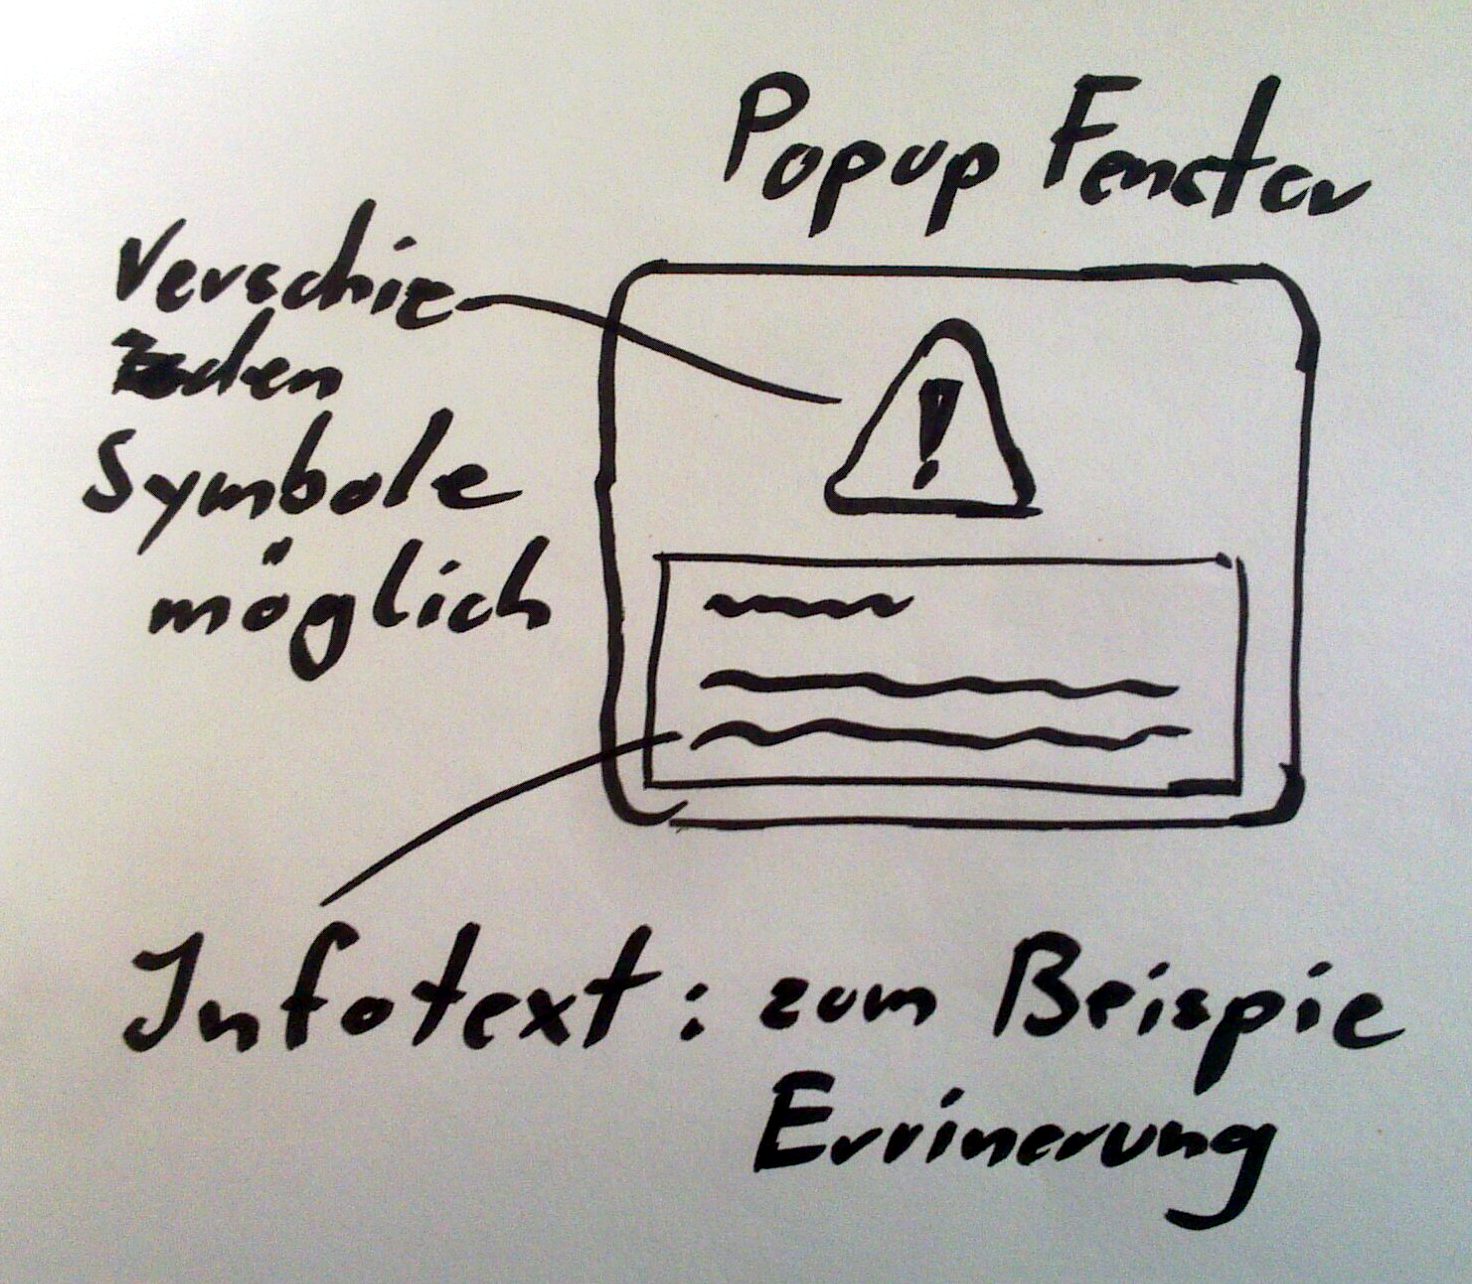
\includegraphics[width = 0.6\textwidth]{../grafiken/popup-fenster}
		\caption{Design Popup Fenster}
	\end{figure}
\end{frame}
%
%
%
\begin{frame}
	\frametitle{Design ListWidget}
%
	\begin{minipage}{0.49\textwidth}
		\begin{figure}
			\centering
			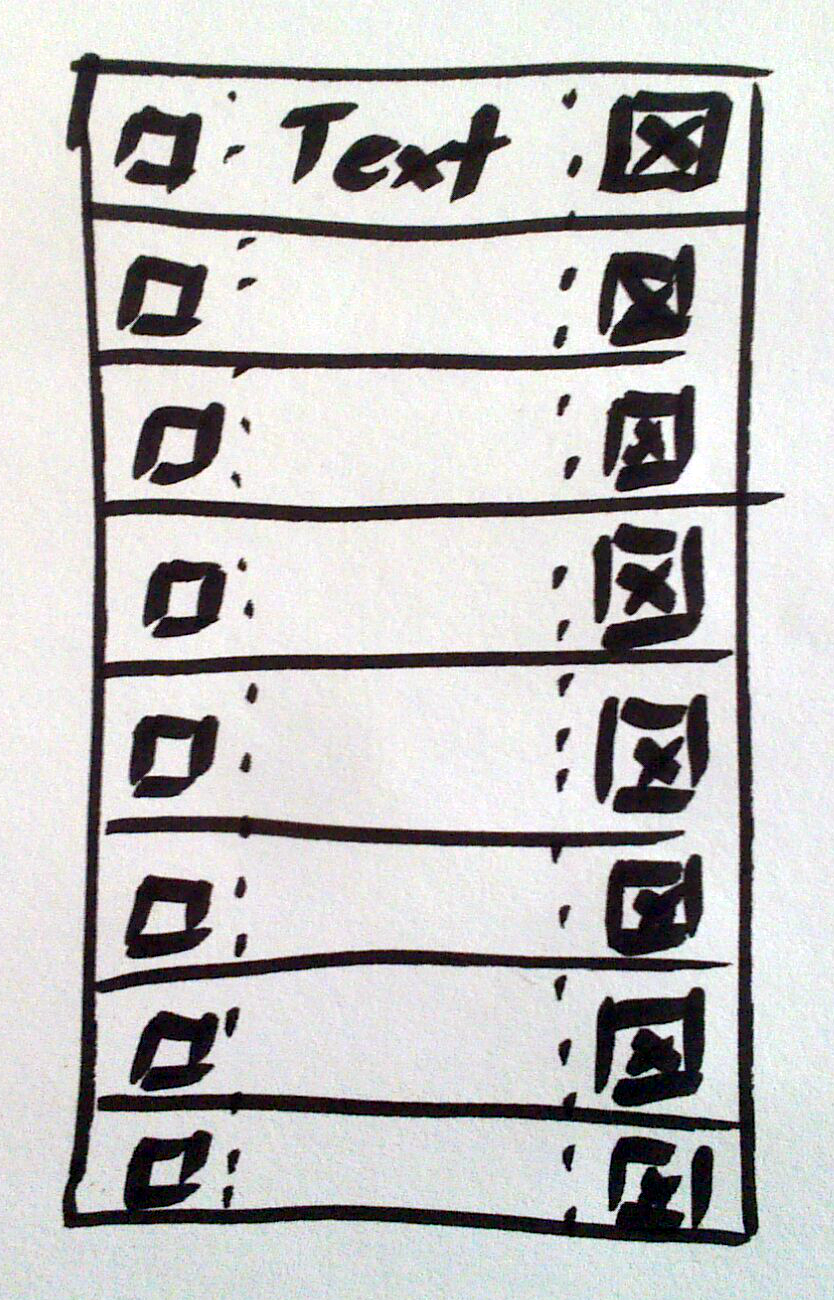
\includegraphics[height = 0.7\textheight]{../grafiken/list-widget-design}
			\caption{Design Checklisten Widget}
		\end{figure}	
	\end{minipage}
%
	\begin{minipage}{0.44\textwidth}
		\begin{block}{ListWidget}
			\begin{itemize}
				\item Enthält zwei Buttons mit Icons
				\item Zwischen den Buttons steht Text
				\item Mit Button rechts, Eintrag löschen
				\item Mit Button links, Eintrag abhacken
			\end{itemize}
		\end{block}
	\end{minipage}
\end{frame}
%
%
%
\begin{frame}
	\frametitle{Anpassung Klassenstruktur ListWidget}
%
	\begin{figure}
		\centering
		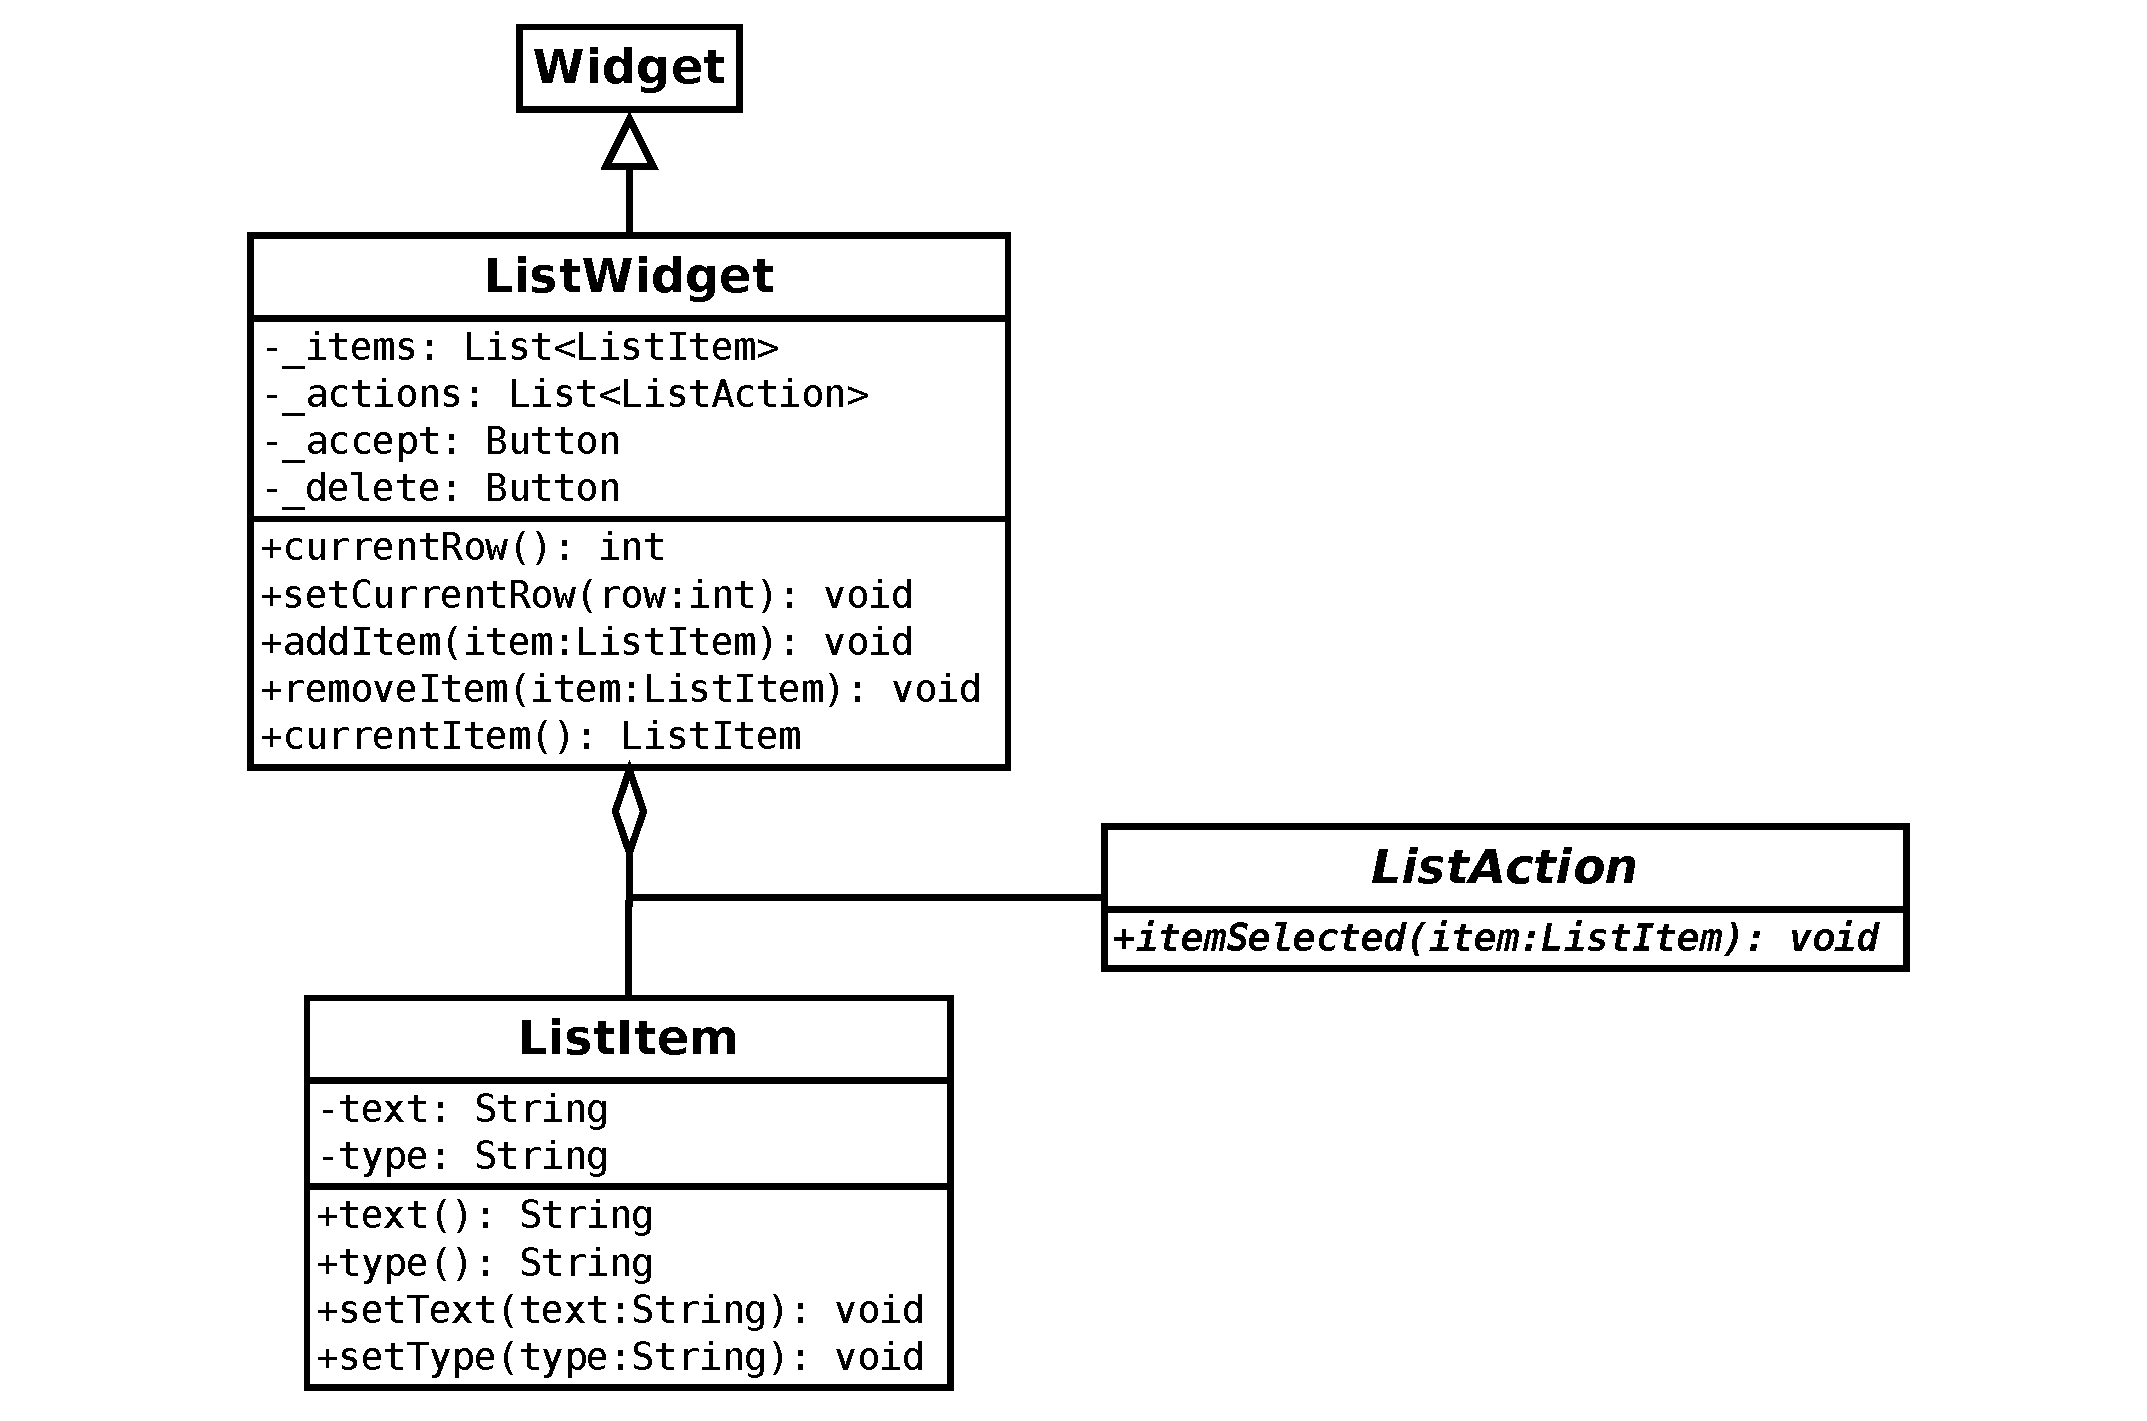
\includegraphics[width = 0.7\textwidth]{../grafiken/uml-list-widget-2}
		\caption{Anpassung der ListWidget}
	\end{figure}
\end{frame}
%
%
%
\begin{frame}
	\frametitle{Google Map API}
%
	\begin{block}{GUI}
		Alles fertig Implementiert in MapView der Google Map API
	\end{block}
\end{frame}